\chapter{Методы прогнозирования}

Под прогнозированием, в широком смысле, понимают вероятностное предположение о состоянии определенного явления в будущем, основанное на специальном научном исследовании~\cite{aliref12}.
Необходимо различать два взаимосвязанных понятия -- метод прогнозирования и модель прогнозирования.

\textit{Метод} прогнозирования представляет собой последовательность действий, которые нужно совершить для получения модели прогнозирования временного ряда~\cite{myref12}.

\textit{Модель} прогнозирования есть представление зависимости будущего значения от прошлого~\cite{myref9, myref13},
при этом способ задания этой зависимости может быть различным.
В некоторых моделях учитывается влияние внешних факторов --- процессов,
протекающих параллельно с исследуемым и влияющих на него.
Внешние факторы могут быть дискретными (представленными временными рядами) или категориальными
(представленными множеством групп)~\cite{myref9, poliref9, poliref10},
при работе с которыми определяют принадлежность значения временного ряда к одной из групп.
Далее в работе будем обозначать внешние факторы как $X(t)$.

В соответствии со способом задания зависимости между будущими и фактическими значениями временного ряда, а также внешними факторами выделяют следующие виды моделей: статистические и структурные.

В \textit{статистических} моделях данная зависимость \textit{задана аналитически}~\cite{myref9}.

К статистическим относятся следующие группы моделей:

\begin{itemize}
\item регрессионные;
\item авторегрессионные;
\item экспоненциального сглаживания~\cite{myref9}.
\end{itemize}

В \textit{структурных} моделях зависимость будущего значения от прошлого задается в виде некоторой \textit{структуры} и правил \textit{перехода} по ней~\cite{myref9, myref13}.

К структурным относятся следующие группы моделей:

\begin{itemize}
\item нейросетевые;
\item на базе цепей Маркова;
\item на базе классификационно -- регрессионных деревьев~\cite{myref9}.
\end{itemize}

Необходимо отметить, что названия моделей и соответствующих методов как правило совпадают~\cite{myref9}.

На основе полученных и хранимых данных прогнозируется дальнейшее поведение временных рядов.

В нашей работе будут рассмотрены следующие методы:

\begin{itemize}
\item модель экспоненциального сглаживания;
\item модель на цепях Маркова;
\item регрессионная модель:
    \begin{itemize}
        \item простая линейная регрессия;
        \item множественная регрессия;
        \item нелинейная регрессия;
    \end{itemize}
\item авторегрессионные модели:
\begin{itemize}
    \item ARIMAX;
    \item GARCH;
    \item ARDLM;
    \item модель по выборке максимального подобия;
\end{itemize}
\item модель на классификационно -- регрессионных деревьях(CART)~\cite{myref9}.
\end{itemize}

\section{Модель экспоненциального сглаживания}

Для того, чтобы прогнозирующая система, включающая тот или иной математический аппарат,
могла автоматически распознавать изменения параметров модели, используется метод экспоненциального сглаживания.

С этой целью применяется сглаженная функция наблюдений:
\begin{equation}
    \label{exp}
    \hat{z_t} = a \cdot z_t + (1 - a) \cdot \widehat{z}_{t-1}.
\end{equation}

Операция~(\ref{exp}), выполняемая при каждом новом наблюдении, называется экспоненциальным сглаживанием.
Значение $a$, которое примерно равно $1/n$, называется коэффициентом сглаживания.
Поскольку операция~(\ref{exp}) проводится одинаково для всех значений ряда динамики, возможно выразить учет более ранних значений в виде:
\begin{multline}
    \label{exp1}
    \hat{z_t} = a \cdot z_t + (1 - a) \cdot (a \cdot z_{t-1} + (1 - a) \cdot \widehat{z}_{t-1}) =\\
    = a \cdot z_t + (1 - a) \cdot (a \cdot z_{t-1} + (1 - a) \cdot(a \cdot z_{t-2} + (1 - a) \cdot \widehat{z}_{t-3})) =\\
    = \ldots = a \cdot \sum_{k=1}^{t-1}(1-a)^k \cdot z_{t-k} + (1-a)^t \cdot z_0.
\end{multline}

Таким образом, сглаженное значение $\hat{z_t}$ представляет собой линейную комбинацию всех значений ряда динамики,
при этом их веса уменьшаются по геометрической прогрессии со временем.

\section{Регрессионная модель}

Регрессионная модель базируется на концепции регрессии, которая представляет собой статистическую зависимость
математического ожидания одной случайной величины от значений другой или нескольких случайных величин.
Основная цель при построении регрессионной модели заключается в обнаружении связи между исходной переменной и несколькими регрессорами (факторами).
В данной работе будут рассмотрены следующие виды регрессионных моделей:
\begin{itemize}[label*=---]
    \item простая линейная регрессия;
    \item множественная регрессия;
    \item нелинейная регрессия.
\end{itemize}

\subsection{Простая линейная регрессия}

Модель основана на предположении о существовании дискретного внешнего фактора $X(t)$, который влияет на рассматриваемый процесс $Z(t)$, и связь между этим фактором и процессом описывается в виде линейной функции. Уравнение для модели прогнозирования временного ряда на основе линейной регрессии представляет собой:
\begin{equation}
    Z(t) = a_0 + a_1 \cdot X(t) + \varepsilon_t,
\end{equation}
где $a_0$, $a_1$ --- коэффициенты регрессии; $\varepsilon_t$ --- ошибка модели.

Классический метод оценки коэффициентов линейной регрессии строится на методе наименьших квадратов.
Этот метод позволяет найти значения коэффициентов $a_0$ и $a_1$, при которых сумма квадратов разностей между фактическими значениями $Z$ и предсказанными значениями $Z_t$ будет минимальной, то есть:
\begin{equation}
    \sum_{i = 1}^{n}(Z_i - Z_{t_i})^2 = \sum_{i = 1}^{n}\varepsilon_i^2 \rightarrow \min
\end{equation}

\subsection{Множественная регрессия}
Для прогнозирования значений процесса $Z(t)$ в момент времени $t$ необходимо иметь значение $X(t)$ для того же времени, что в реальности часто бывает сложно.
На практике процесс $Z(t)$ может зависеть от множества дискретных внешних факторов $X_1(t),\ldots,X_s(t)$.
Таким образом, модель прогнозирования принимает следующий вид:
\begin{equation}
    Z(t) = a_0 + a_1 \cdot X_1(t) + a_2 \cdot X_2(t) + \ldots + a_s \cdot X_s(t) + \varepsilon_t,
\end{equation}
$a_0, a_1, \ldots, a_s$ --- коэффициенты регрессии; $\varepsilon_t$ --- ошибка модели.

Коэффициенты регрессии также определяются с использованием метода наименьших квадратов, но в этом случае решается система нормальных уравнений, определитель которой выглядит как:
\begin{equation}
    \begin{vmatrix}
        n & \sum X_1 & \ldots & \sum X_s^2 \\
        \sum X_1 & \sum X_1^2 & \ldots & \sum X_1X_s \\
        \ldots & \ldots & \ldots & \ldots \\
        \sum X_s & \sum X_1X_s & \ldots & \sum X_s^2
    \end{vmatrix}
\end{equation}

\subsection{Нелинейная регрессия}

Нелинейная модель предполагает существование определенной функции:
\begin{equation}
    Z(t) = F(X(t), A),
\end{equation}
где $Z(t)$ --- исходный процесс;
$X(t)$ --- внешний фактор, от которого зависит процесс $Z(t)$;
$A$ --- функция, параметры которой необходимо определить в рамках построения модели прогнозирования.

На практике нелинейные регрессионные модели применяются редко, поскольку лишь небольшая часть процессов имеет известную заранее функциональную зависимость~\cite{aliref3}.

\section{Авторегрессионные модели прогнозирования}

\subsection{Модель прогнозирования ARIMAX}

1. Авторегрессия $p$-го порядка $AR(p)$ --- это модель временного ряда, в которой его прогнозируемое значение является
линейной комбинацией конечного числа предыдущих значений этого ряда и белого шума~\cite{myref9,poliref8}.

\begin{equation}
    \label{a1}
    Z(t) = \sum_{i=1} ^{p} \alpha_i \cdot Z_{t-i}+\epsilon_t,
\end{equation}

где $p$ --- число значений ряда, учитываемых в модели (порядок модели);
$\alpha_i$~--- коэффициенты модели, их требуется оценить при построении;
$\epsilon_t$~--- белый шум –- случайная составляющая, которая не может быть объяснена предыдущими значениями временного
ряда и используется для оценки точности прогнозов~\cite{poliref8}.

2. Модель скользящего среднего $q$-го порядка $MA(q)$ — модель временного ряда, в которой его прогнозируемое значение
является линейной комбинацией конечного числа предыдущих значений белого шума~\cite{poliref3, poliref8}.

\begin{equation}
    Z(t) = \epsilon_t+\sum_{j=1} ^{q} b_j \cdot \epsilon_{t-j},
\end{equation}

где $b_j$ ---  параметры модели;
$\epsilon$ --- белый шум.

3. $ARMA(p, q)$ модель включает в себя авторегрессию $p$-го порядка $AR(p)$ и модель скользящего среднего $q$-го порядка $MA(q)$~\cite{myref9, poliref8}.
4. При \textbf{ARIMA} требуется произвести следующие действия~\cite{myref9}:
\begin{enumerate}
    \item выявить наличие единичных корней;
    \item определить порядок интегрированности временного ряда;
    \item если порядок интегрированности больше нуля:
    \begin{enumerate}
        \item[3.1)] преобразовать ряд взятием разности (обычно равна значению белого шума) соответствующего порядка;
        \item[3.2)] построить ARMA-модель для преобразованной стационарной модели.
    \end{enumerate}
\end{enumerate}

\textbf{Модель прогнозирования ARIMAX} (AutoRegressive Integrated Moving Average eXtended) --- это математическая модель для анализа временных рядов,
объединяющая в себе интегрированную авторегрессию, скользящее среднее и возможность учета внешних факторов (exogenous factors)~\cite{myref9, poliref8}.

\subsection{Модель прогнозирования GARCH}
Прогнозирование с использованием авторегрессионной модели с условной гетероскедастичностью (GARCH) происходит следующим образом~\cite{myref9, poliref8}:
\begin{enumerate}
    \item определить модель $AR(p)$ для исходного временного ряда~(\ref{a1});
    \item взять ошибку (белый шум) модели~(\ref{a1}) $\epsilon_t$ равным:
\end{enumerate}

\begin{equation}
    \epsilon_t = \sigma_t \cdot v_t,
\end{equation}
где $\sigma_t$ --- зависимое от времени стандартное отклонение;
$v_t$ --- величина, с нормальным распределением, среднее значение равно 0, и стандартное отклонение равно 1.

\begin{equation}
    \label{pol5}
    \sigma_t^2 = b_0+b_1 \cdot \epsilon_{t-1}^2 + \ldots + b_q \cdot \epsilon_{t-q}^2 + c_1 \cdot \sigma_{t-1}^2 +  \ldots + c_p \cdot \sigma_{t-p}^2,
\end{equation}
где $b_i$ и $c_i$ --- коэффициенты.

Уравнение~(\ref{pol5}) называется моделью $GARCH(p, q)$.
$p$ – характеризует порядок авторегрессии квадратов остатков;
$q$ — количество предшествующих оценок остатков~\cite{myref9, poliref8}.

\subsection{Модель прогнозирования ARDLM}

При моделировании процессов на изучаемую переменную могут влиять не только текущие значения процесса, но и его лаги,
то есть значения временного ряда, предшествующие изучаемому моменту времени~\cite{myref9, poliref8}.
Например, для переменной $z_t$ лагом в $k$ периодов будет $z_{t-k}$.

При работе с временными рядами удобно использовать лаговый оператор L --– оператор сдвига назад во времени~\cite{poliref8}:

\begin{equation}
   L^m \cdot z_t = z_{t-m},
\end{equation}
где $m$ --- количество периодов задержки (величина лага).

Модель авторегрессии распределенного лага ARDLM(p, l) описывается уравнением~\cite{poliref8}:
\begin{equation}
    Z(t) = \varphi_0+\varphi_1Z(t-l-1)+\ldots+\varphi_pZ(t-l-p)+\epsilon_t,
\end{equation}
где $\varphi_i$ --- количество периодов задержки (величина лага);
$\epsilon_t$ --- белый шум;
$l$ --- величина лага.

\subsection{Модель по выборке максимального подобия EMMSP}

Для удобства анализа данной модели временной ряд обозначают как $Z_1^N=(z_1,z_2,\ldots,z_N)$.
Набор из $M$ последовательных значений \newline $Z_t^M=(z_t,z_{t+1},\ldots,z_{t+M-1})$, лежащих внутри временного ряда $Z_1^N$,
назовют \textit{выборкой} из этого ряда длины $M\in[1,(N-1)]$ с моментом начала отсчета $t\in[1,(N-M)]$.
Разность начал отсчетов выборок $Z_t^M$ и $Z_{t-k}^M$ называют \textit{задержкой} $k\in[1,(t-1)]$.

Выборки обладают свойством подобия, что используют для прогнозирования временного ряда~\cite{myref9}.
Идея метода заключается в построении ожидаемой выборки с помощью аппроксимации уже существующей.
С целью реализации данной технологии следует ответить на следующие вопросы.

1. Как аппроксимировать выборки?

Необходимо рассмотреть аппроксимацию выборки \newline $Z_{T-M+1}^M$ при помощи выборки $Z_{T-M+1-k}^M$~\cite{myref9}.
Далее момент времени обозначен $T-M+1=t$.

Аппроксимированные значения выборки $\widehat{Z}_t^M$ вычисляются следующим образом:

\begin{equation}
    \widehat{Z}_t^M = \alpha_1Z_{T-k}^M+\alpha_0I^M,
\end{equation}
где $\alpha_1$ и $\alpha_0$ --- коэффициенты,
а $I^M$ - единичный вектор размерности $M$.

Согласно методу наименьших квадратов, коэффициенты аппроксимации определяются, исходя из уравнения

\begin{equation}
    Z_x \cdot A = Z_y,
\end{equation}

где $Z_x$ и $Z_y$ определяются следующим образом:
\begin{flushright}
\begin{equation}
    Z_X =
\begin{pmatrix}
           \sum_{i=0}^{M-1} Z^2(k+1) & \sum_{i=0}^{M-1} Z(k+i) \\
           \sum_{i=0}^{M-1} Z(k+1)   & M
\end{pmatrix};

    Z_Y =
    \begin{pmatrix}
               \sum_{i=0}^{M-1} Z(k+i) \cdot Z(T-M+1+i) \\
               \sum_{i=0}^{M-1} Z(T-M+1+i)
\end{pmatrix}.{\qquad\qquad }
    \label{eq:equation}
\end{equation}
\end{flushright}

2. Какую выборку следует аппроксимировать?

Подходящую для аппроксимации выборку называют \textit{базовой историей}~\cite{myref9}.
Она располагается на оси времени сразу за \textit{выборкой максимального подобия} для новой истории $Z_{T-M+1}^M$~\cite{myref9}.
Новая история содержит значения процесса непосредственно перед моментом прогноза.
Соответственно, чтобы вычислить базовую историю, следует определить выборку максимального подобия.

3. Как определить выборку максимального подобия для выборки новой истории?

Как следует из названия, мы ищем такую выборку, значения которой являются наиболее близкими к значениям новой истории.
Отсюда, необходимо ввести меру подобия двух выборок.
Введем коэффициент $\rho$.
Он зависит от длины $M$ выборок, а также от задержки $k$, и характеризует степень линейной зависимости указанных выборок:
чем ближе к единице значение $\rho$, тем выше их линейная зависимость~\cite{myref9, myref11}.

Далее необходимо рассмотреть все возможные выборки длины $M$ и вычислить для них коэффициент подобия новой истории.
Выборка с максимальным значением $\rho$ и будет выборкой максимального подобия.
Данной выборке соответствует задержка $k$, которую далее обозначим как $kmax$.

В результате получаем функциональную зависимость значений прогнозируемой выборки $Z_t^P$ от фактически существующей $Z_{T-k}^M$~\cite{myref9}:

\begin{equation}
    \widehat{Z}_t^P = \alpha_1Z_{k_{max}+M}^P+\alpha_0I^P=EMMSP(M),
\end{equation}

На рисунке~\ref{img2} приведен пример расположения рассмотренных для прогнозирования выборок.
\begin{figure}[h]
    \centering
    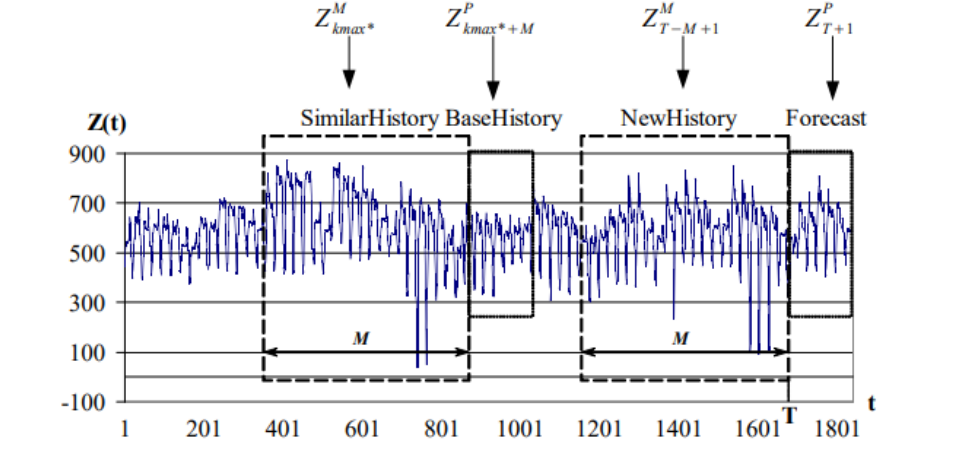
\includegraphics[scale=0.7]{img/img2}
    \caption{Положение выборок для прогнозирования временного ряда с помощью модели по выборке максимального подобия без учета внешних факторов~\cite{myref9}}
    \label{img2}
\end{figure}

Кроме того, существует возможность построить модель, учитывающую внешние факторы,
которые также представлены в виде временного ряда со значениями, соответствующими отметкам времени временного ряда $Z$.
В данной модели отличается процесс аппроксимации выборок, в остальном алгоритм прогнозирования аналогичен уже рассмотренному.

Функциональная зависимость значений прогнозируемой выборки $Z_t^P$ от фактически существующей $Z_{T-k}^M$,
с учетом внешних факторов $X$, будет выглядеть следующим образом~\cite{myref9}:

\begin{equation}
    \widehat{Z}_{T+1}^P = \alpha_2Z_{k_{max^*+M}+M}^P+\alpha_0I^P+\alpha_1X_{T+1}^P=EMMSP(M),
\end{equation}

На рисунке~\ref{img3} представлены выборки для модели с учетом внешних факторов.
\begin{figure}[h]
    \centering
    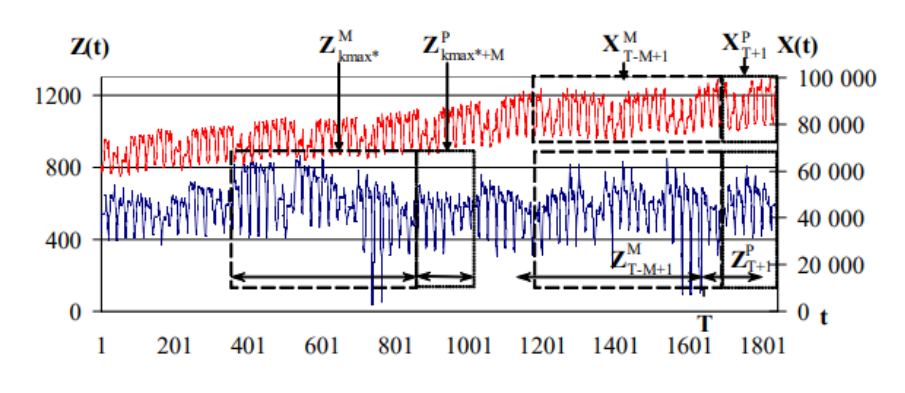
\includegraphics[scale=0.8]{img/img3}
    \caption{Положение выборок для прогнозирования временного ряда с помощью модели по выборке максимального подобия с учетом внешних факторов~\cite{myref9}}
    \label{img3}
\end{figure}


Подводя итоги, можно выделить основные этапы алгоритма построения модели по выборке максимального подобия.

Необходимо вычислить:
\begin{enumerate}
    \item выборку новой истории;
    \item выборку максимального подобия;
    \item выборку базовой истории;
    \item прогнозные значения.
\end{enumerate}

Рассмотрев метод прогнозирования по выборке максимального подобия, можно выделить следующие особенности его применения:

\begin{itemize}
    \item модель работает с неравноотстоящими временными рядами;
    \item модель применяется для стационарных и нестационарных временных рядов;
    \item количество итераций (1шт.) для вычисления прогноза не зависит от требуемого количества элементов прогнозируемой выборки;
    \item модель имеет единственный параметр $M$ --- длина выборки, от которого зависит значение прогнозируемого участка, в отличие от других авторегрессионных моделей.
\end{itemize}

\section{Модель на классификационно -- регрессионных деревьях CART}

Структурные модели CART разработаны для моделирования процессов, на которые оказывают влияние как дискретные внешние факторы, так и категориальные.
Если внешние факторы, влияющие на процесс $X(t)$, дискретны, то используются регрессионные деревья;
если факторы категориальные, то -- классификационные деревья.
В случае, если необходимо учитывать факторы обоих типов, то используются смешанные классификационно -- регрессионные деревья~\cite{myref9, poliref11}.

\begin{figure}[h]
    \centering
    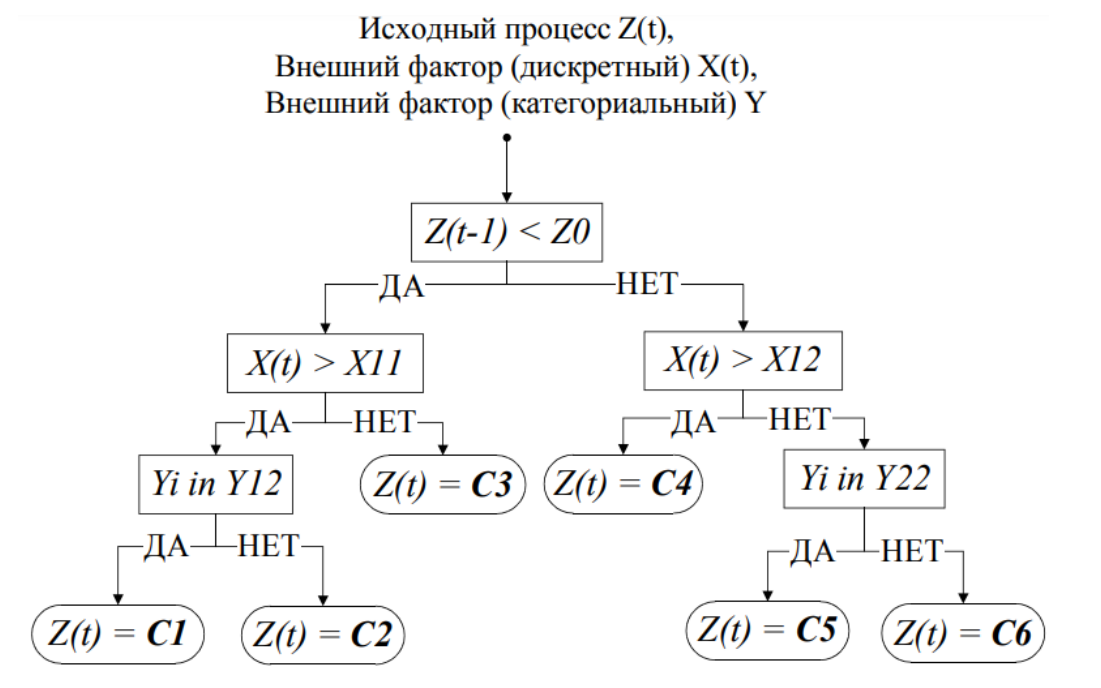
\includegraphics[scale=0.7]{img/tree}
    \caption{Бинарное классификационно -- регрессионное дерево}
    \label{tree}
\end{figure}

Согласно модели CART, прогнозное значение временного ряда зависит от предыдущих значений, а также некоторых независимых переменных.

На рисунке~\ref{tree} рассматривается пример классификационно -- регрессионного дерева, прогнозирование по такому дереву протекает следующим образом:

\begin{enumerate}
    \item предыдущее значение процесса сравнивается с константой $X_0$;
    \item если $Z(t-1)<Z_0$, то
    \begin{enumerate}
        \item[2.1)] если $X(t)\leqslantX_{11}$, то $Z(t)=C_3$, иначе
        \begin{enumerate}
                  \item[2.1.1)] если $Y_i\inY_{12}$, то $Z(t)=C_3$, иначе $Z(t)=C_2$;
        \end{enumerate}
    \end{enumerate}
    иначе
    \begin{enumerate}
        \item[2.2)] если $X(t)>X_{12}$, то $Z(t)=C_4$, иначе
        \begin{enumerate}
            \item[2.2.1)] если $Y_i\inY_{22}$, то $Z(t)=C_5$, иначе $Z(t)=C_6$.
        \end{enumerate}
    \end{enumerate}
\end{enumerate}

При определении значения учитываются как дискретные внешние факторы $X(t)$, так и категориальные $Y$,
для которых выполняется проверка принадлежности значения в одном из заранее определенных подмножеств.

Значения пороговых констант, $Z_0$, $X_{11}$, а также подмножеств $Y_{12}$, $Y_{22}$ определяются на этапе построения дерева.

Таким образом был описан метод прогнозирования временного ряда посредством классификационно -- регрессионных деревьев.
Для использования этого метода необходимо указать алгоритм построения бинарного дерева решений
(дихотомической классификационной модели) --- CART (Classification and Regression Tree).
Его суть заключается в рекурсивном делении исходного набора данных на подмножества, которые становятся все более и
более однородными относительно выделенных признаков, в результате чего формируется древовидная иерархическая структура,
где каждый узел дерева имеет только двух потомков~\cite{poliref11, poliref12, poliref13, poliref14}.

Построение дерева происходит следующим образом~\cite{poliref11, poliref12, poliref13, poliref14}:

1) выбрать атрибут, который должен разбить множество наблюдений в узле так,
чтобы результирующие подмножества содержали элементы, принадлежащие одному классу или количество «примесей» было минимально.

2) оценить правильность выбора атрибута разбиения используется индекс Джини, лучшим будет то разбиение,
для которого значение индекса Джини будет минимальным.
Индекс рассчитывается по формуле:

\begin{equation}
    Gini(Q)=1-\sum_{i=1} ^{n} p_i^2,
\end{equation}
где $Q$ --- результирующее множество;
$n$ --- число классов в нем;
$p_i\in[0,1]$ --- относительная частота элементов множества, принадлежащих $i$-му классу
(принимает 0 – если все элементы  относятся к одному классу,
1 – когда классы представлены в равных пропорциях и равновероятны).

3) определить и оценить новый атрибут в случае некорректного выбора;

4) преобразовать предков «пустого» (куда не попал ни один элемент) узла в лист, если был сформирован таковой.

Построение дерева приходится повторять для каждого следующего прогнозируемого значения.
Из-за высокой погрешности прогнозирования данный метод не подходит для долгосрочного прогнозирования~\cite{poliref11, poliref12, poliref13, poliref14}).

\section{Модель на цепях Маркова}

\textit{Цепь Маркова} --- это математическая модель, которая используется для моделирования случайных процессов,
происходящих в течение определенного периода времени~\cite{myref8, myref9, myref13, myref16}.
Она состоит из набора состояний и переходов между ними~\cite{myref16, myref9}.
Возможность перехода из одного состояния в другое зависит исключительно от текущего состояния, а не от каких-либо прошлых событий.
Данное условие также называют марковским свойством процесса~\cite{myref8, myref9,myref13, myref16}.

Пример цепи Маркова для процесса, имеющего три состояния, представлен на рисунке~\ref{chain}, где $S1$, $S2$, $S3$ — состояния процесса $Z(t)$,
а вероятность перехода из состояния:
\begin{itemize}
    \item S1 в S2 равна 0.5,
    \item S2 в S1 равна 0.0,
    \item S1 в S3 равна 0.25,
    \item S3 в S2 равна 0.33 и так далее.
\end{itemize}

\begin{figure}[h]
    \centering
    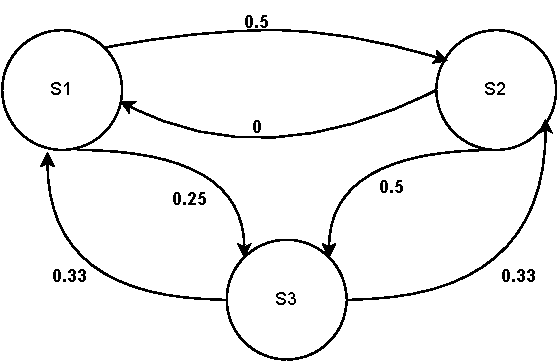
\includegraphics[scale=1.1]{img/chain}
    \caption{Цепь Маркова}
    \label{chain}
\end{figure}

Для расчета динамики цепи достаточно рассмотреть два аспекта:
\begin{itemize}
    \item \textit{вектор исходного распределения вероятностей} $A$ ---
    вектор, каждое $i$-ое значение в котором, соответствует вероятности того, что система находится в $i$-ом состоянии~\cite{myref1}.
    Например, для модели из трех состояний:
    \begin{equation}
        A = (0.0, 0.5, 0.5);
        \label{eq:equation2}
    \end{equation}
    \item матрицу переходных вероятностей $P$, представляющую собой матрицу, каждое значение $(i, j)$ которой
    соответствует вероятности того, что элемент перейдет из состояния $s_i$ в состояние $s_j$ на следующем шаге процесса~\cite{myref1}.
    Например, для модели на рисунке выше:
    \begin{equation}
        P = \begin{pmatrix}0.25, 0.50, 0.25\\
                    0.00, 0.50, 0.50\\
                    0.33, 0.33, 0.33
                \end{pmatrix}.
        \label{eq:equation3}
    \end{equation}
\end{itemize}

Чтобы определить вектор распределения вероятностей на следующем шаге необходимо вычислить произведение вектора $A$ и матрицы $P$~\cite{myref13}.
Для рассматриваемого примера:

\begin{equation}
    (0.00, 0.50, 0.50) = \begin{pmatrix}0.25, 0.50, 0.25\\
    0.00, 0.50, 0.50\\
    0.33, 0.33, 0.33
    \end{pmatrix}=(0.165, 0.415, 0.420).
\label{eq:equation4}
\end{equation}

Следовательно, вероятность того, что цепь находится в состоянии $s_i$ после $n$ шагов, является $i$-ой записью в векторе~\cite{myref1}:
\begin{equation}
    A_n = A_{n-1}P.
    \label{eq:equation5}
\end{equation}

Основные этапы алгоритма построения модели временного ряда на цепях Маркова:
\begin{enumerate}
    \item выделить состояния временного ряда;
    \item проверить, можно ли считать рассматриваемый процесс Марковским;
    \item вычислить матрицу переходных вероятностей;
    \item определить вероятностный вектор, представляющий некоторое начальное распределение;
    \item вычислить произведение матрицы и вектора n раз для получения вектора распределения вероятностей.
\end{enumerate}

Рассмотрев метод прогнозирования на цепях Маркова, можно выделить следующие особенности его применения:
\begin{itemize}
    \item необходимо выделить состояния временного ряда.
    Данное действие является дополнительным и зависит от сферы применения временного ряда;
    \item прогнозируемый ряд должен являться Марковским процессом;
    \item единообразие анализа и проектирования~\cite{myref9}.
\end{itemize}

\section{Сравнение методов прогнозирования временных рядов}

Результаты классификации методов прогнозирования временных рядов приведены в таблицах~\ref{tab_prog1} и~\ref{tab_prog2}.

\begin{table}[h!]
    \caption{Классификация методов прогнозирования временных рядов (часть 1)}
    \label{tab_prog1}
    \centering
    \rotatebox{90}{
        \begin{tabular}{||p{3cm}||p{2cm}|p{2cm}|p{2cm}|p{2cm}|p{2cm}|p{2cm}|p{2cm}|p{1cm}||}
            \hline
            & \multicolumn{8}{ c|}{методы прогнозирования} \\ \cline{2-9}
            \multirow{2}{4cm}{классифика- ционный параметр} & {на цепях Маркова} & {на классификационно -- регрессионных деревьях} & {экспонен- циального сглаживания} & \multicolumn{3}{ c|}{регрессионные} & \multicolumn{2}{ c|}{авторегрессионные}\\
            {} & {} & {} & {} & {простая линейная} & {множе- ственная линейная} & {нелиней- ная} & {ARIMAX, GARCH, ARDLM} & {EMMSP}\\
            \hline
            \hline
            {тип модели} & \multicolumn{2}{ c|}{структурная} & \multicolumn{6}{ c||}{статистическая}\\
            \hline
            {необходимость преобразовывать данные временного ряда перед их прогнозированием} & {надо выделить состояния модели} & {надо построить дерево} & \multicolumn{6}{ c||}{не надо}\\
            \hline
            {количество учитываемых внешних факторов} & {любое} & {любое} & {0} & {1} & {любое} & {1} & {любое} & {1}\\
            \hline
            {тип учитываемых внешних факторов} &  \multicolumn{2}{p{2cm}|}{категориальные и дискретные} & \multicolumn{6}{c|}{только дискретные}\\
            \hline\hline
        \end{tabular}}
\end{table}
\clearpage

\begin{table}[h!]
    \caption{Классификация методов прогнозирования временных рядов (часть 2)}
    \label{tab_prog2}
    \centering
    \rotatebox{90}{
        \begin{tabular}{||p{3cm}||p{2cm}|p{3cm}|p{1.5cm}|p{2cm}|p{2cm}|p{2cm}|p{2cm}|p{2cm}||}
            \hline
            & \multicolumn{8}{ c|}{методы прогнозирования} \\ \cline{2-9}
            \multirow{2}{4em}{классифика- ционный параметр} & {на цепях Маркова} & {на классификационно -- регрессионных деревьях} & {экспо- ненциального сглаживания} & \multicolumn{3}{ c|}{регрессионные} & \multicolumn{2}{c|}{авторегрессионные}\\
            {} & {} & {} & {} & {простая линейная} & {множе- ственная линейная} & {нелиней- ная} & {ARIMAX, GARCH, ARDLM} & {EMMSP}\\
            \hline
            \hline
            {область применения} & {неприме- нима к долгохранимым или не выполняющим Марковское свойство временным рядам} & {необходи- ма возможность принятия решения, когда стоит прекратить дальнейшие ветвления дерева} & {} & \multicolumn{2}{ p{4cm}|}{отсутствие возможности моделирования нелинейных процессов} & {процесс должен иметь известную заранее функциональную зависимость} & {} & {неравно- стоящие, стационарные и нестационарные ряды}\\
            \hline\hline
        \end{tabular}}
\end{table}
\clearpage

Подводя итоги, можно заметить, что статистические и структурные модели имеют ряд различий.
Статистические модели не требуют специальной обработки дискретных данных перед применением методов прогнозирования,
в отличие от рассмотренных структурных методов: для цепей Маркова необходимо выделить состояния модели, а в случае
классификационно -- регрессионной модели нужно построить  одноименное дерево.
Данная особенность позволяет учитывать влияние внешних факторов, которые не являются дискретными, что невозможно в рассмотренных статистических моделях.

С точки зрения количества учитываемых внешних дискретных факторов классифицируем методы следующим образом:
\begin{itemize}
    \item без учета внешних факторов:  модель экспоненциального сглаживания;
    \item с учетом одного дискретного внешнего фактора: некоторые типы регрессионных моделей и авторегрессионная модель по выборке максимального подобия;
    \item с учетом любого количества внешних факторов: структурные модели, модель множественной регрессии и большинство авторегрессионных моделей.
\end{itemize}

Все рассмотренные модели имеют различную область применения, поэтому при выборе модели прогнозирования необходимо проверить,
удовлетворяет ли временной ряд упомянутым требованиям.


